\documentclass{article}

\usepackage{tikz}
\usepackage{amsmath}
\usepackage[left=2.3cm, right=2.3cm, top=1.7cm, bottom=1.7cm]{geometry}

\usepackage{Sweave}
\begin{document}
\input{investigation-concordance}

{\Large \textbf{Name:}} \hspace{3cm} \vspace{1cm}

\begin{center}
{\Huge Year 10 Indices Investigation}
\end{center}

{\Large 

\textbf{Part 1A} \\[-6pt]

\begin{center}
\includegraphics{./fractal.png}
\end{center}

The above shows how a fractal is constructed  in stages from left to right. Each stage is constructed from the previous stage by splitting each remaining square into 9 equal squares and removing 4 of them. Stage 0 (the leftmost image) is a $1 \times 1$ square, so it has total area of 1 $\text{unit}^2$.
\vspace{0.4cm}

\textbf{(a)} Explain why stage 1 has a total area of {\huge $\frac{5}{9}$} $\text{unit}^2$.

\vspace{0.4cm}
\begin{center}
\begin{tikzpicture}[scale=0.8]
\draw[black,thin] (0,0) -- (20, 0);
\draw[black,thin] (0,1) -- (20, 1);
\draw[black,thin] (0,2) -- (20, 2);
\draw[black,thin] (0,3) -- (20, 3);
\draw[black,thin] (0,4) -- (20, 4);
\draw[black,thin] (0,5) -- (20, 5);
\draw[black,thin] (0,6) -- (20, 6);
\end{tikzpicture}
\end{center}
\vspace{0.2cm}

\textbf{(b)} Explain why stage 2 has a total area of {\huge $\frac{25}{81}$} $\text{unit}^2$.

\vspace{0.4cm}
\begin{center}
\begin{tikzpicture}[scale=0.8]
\draw[black,thin] (0,0) -- (20, 0);
\draw[black,thin] (0,1) -- (20, 1);
\draw[black,thin] (0,2) -- (20, 2);
\draw[black,thin] (0,3) -- (20, 3);
\draw[black,thin] (0,4) -- (20, 4);
\draw[black,thin] (0,5) -- (20, 5);
\draw[black,thin] (0,6) -- (20, 6);
\end{tikzpicture}
\end{center}
\vspace{0.2cm}


\pagebreak 
{\Large \textbf{Part 1A continued...} \\[6pt]

\textbf{(c)} Write {\huge $\frac{25}{81}$} as a power of {\huge $\frac{5}{9}$}

\vspace{0.1cm}
\begin{center}
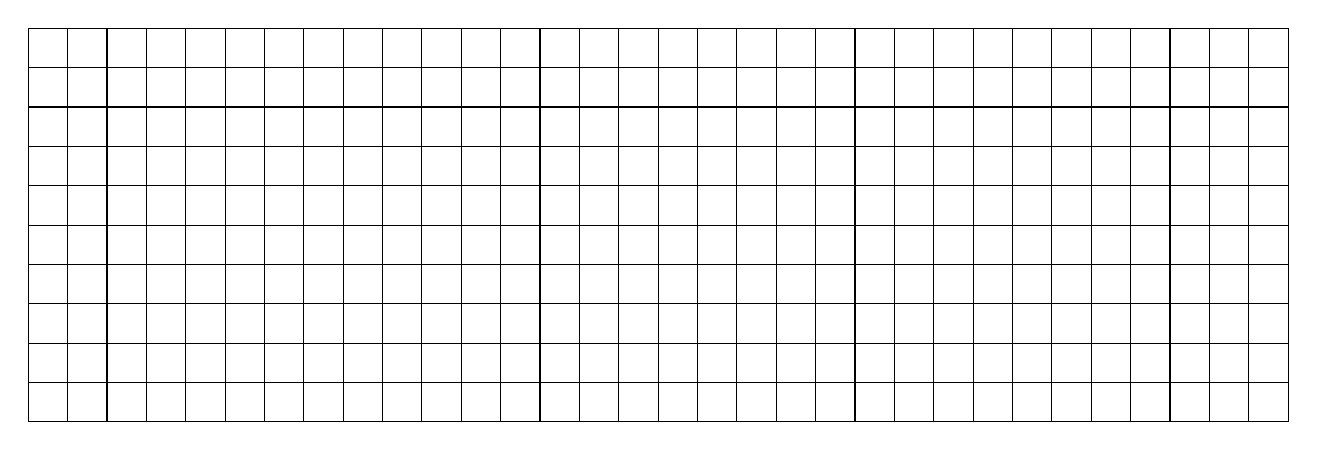
\begin{tikzpicture}
\draw[step=0.5,black,thin] (0,0) grid (16, 5);
\end{tikzpicture}
\end{center}

\textbf{(d)} Write an expression \emph{using indices} to represent the area of Stage 3.

\vspace{0.1cm}
\begin{center}
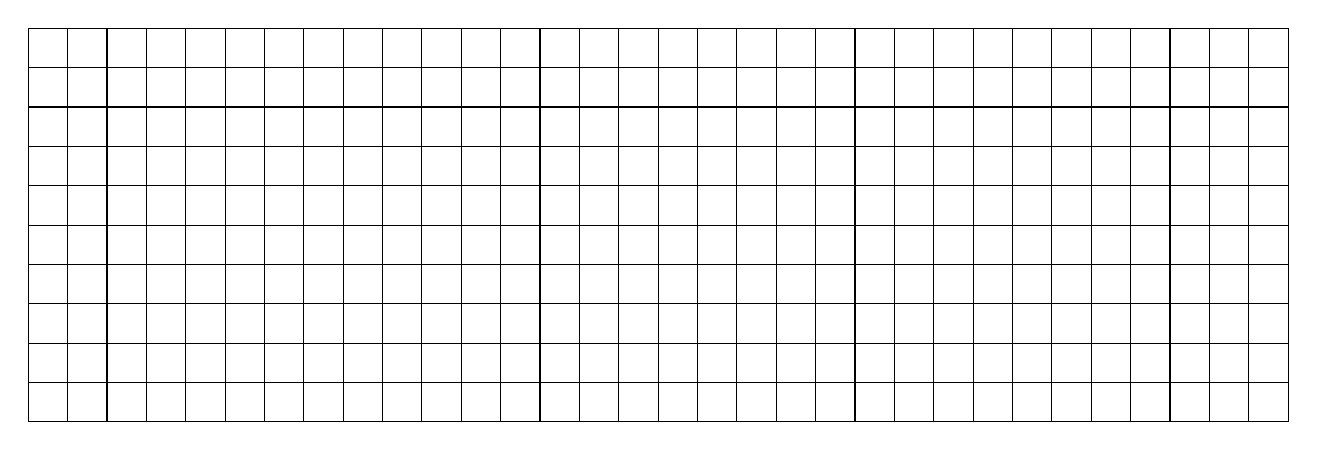
\begin{tikzpicture}
\draw[step=0.5,black,thin] (0,0) grid (16, 5);
\end{tikzpicture}
\end{center}

\textbf{(e)} Hence, or otherwise, write an expression \emph{using indices} to represent the area of Stage $n$.

\vspace{0.1cm}
\begin{center}
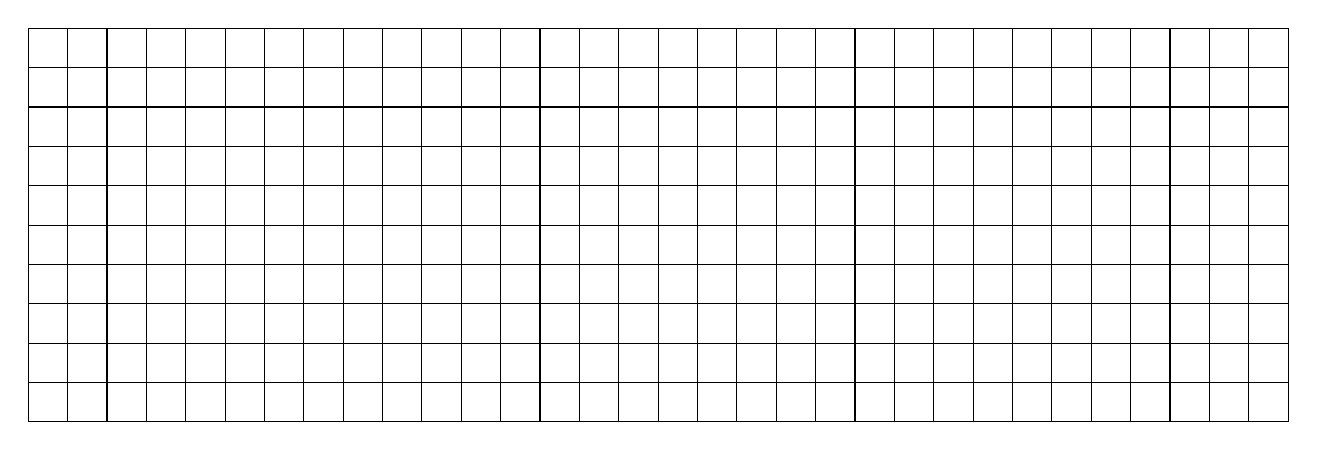
\begin{tikzpicture}
\draw[step=0.5,black,thin] (0,0) grid (16, 5);
\end{tikzpicture}
\end{center}

\pagebreak
\textbf{Part 1B}

The perimeter of stage $0$ is $4$ units. \\[6pt]

\textbf{(a)} Write an expression for the perimeter of stage $1$ as a multiple of the perimeter of stage 0 (so $4$ multiplied by something).  Explain how you arrived at your answer.

\vspace{0.1cm}
\begin{center}
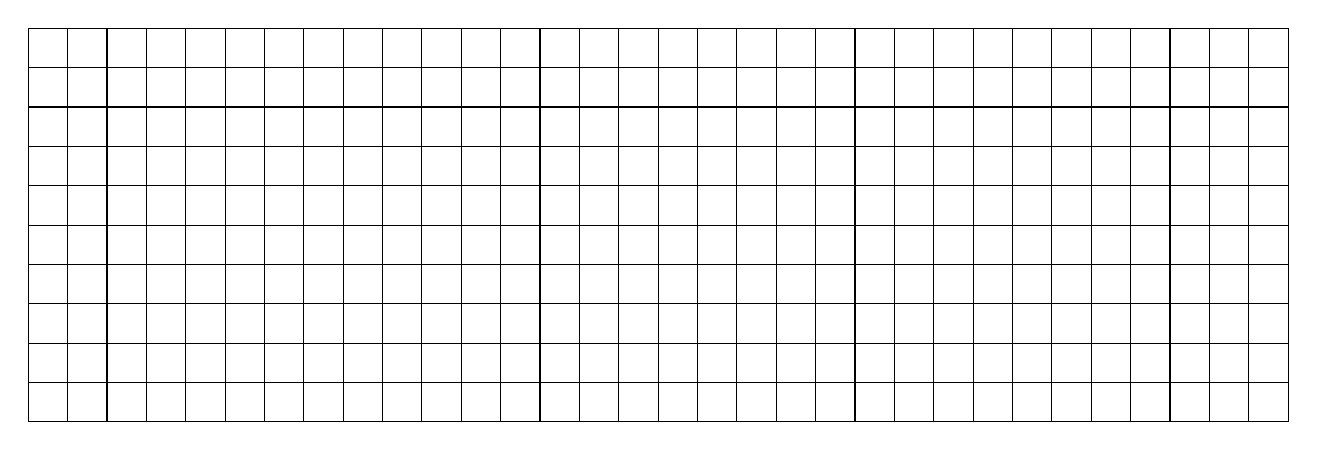
\begin{tikzpicture}
\draw[step=0.5,black,thin] (0,0) grid (16, 5);
\end{tikzpicture}
\end{center}

\textbf{(b)} Write an expression for the perimeter of stage $2$ as a multiple of the perimeter of stage 0 (so $4$ multiplied by something).  Explain how you arrived at your answer.

\vspace{0.1cm}
\begin{center}
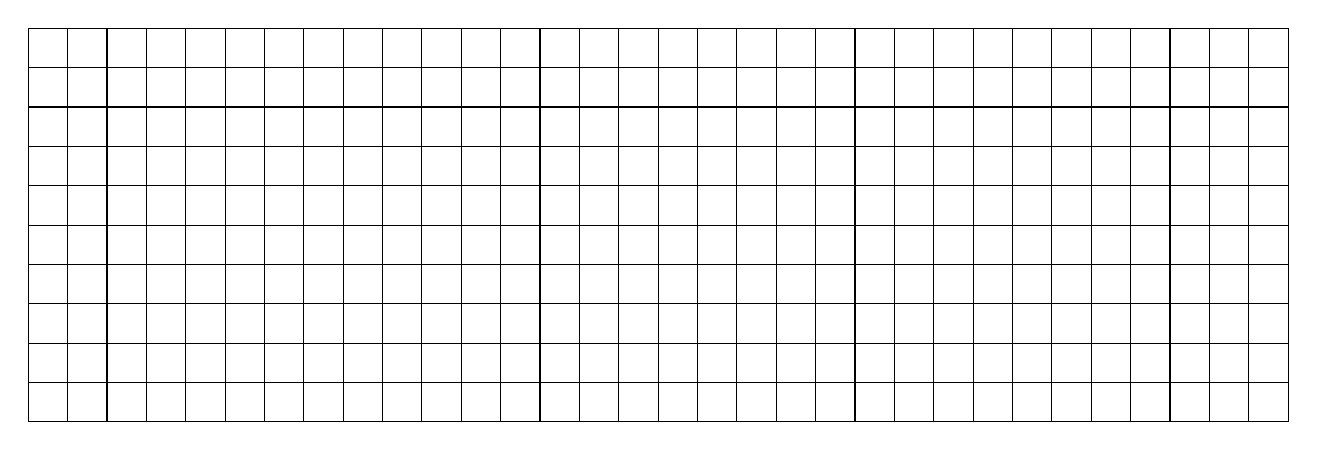
\begin{tikzpicture}
\draw[step=0.5,black,thin] (0,0) grid (16, 5);
\end{tikzpicture}
\end{center}

\pagebreak
{\Large \textbf{Part 1B continued...} \\[6pt]

\textbf{(c)} Write an expression \emph{using indices} for the perimeter of stage $3$ as a multiple of the perimeter of stage 0 (so $4$ multiplied by something).

\vspace{0.1cm}
\begin{center}
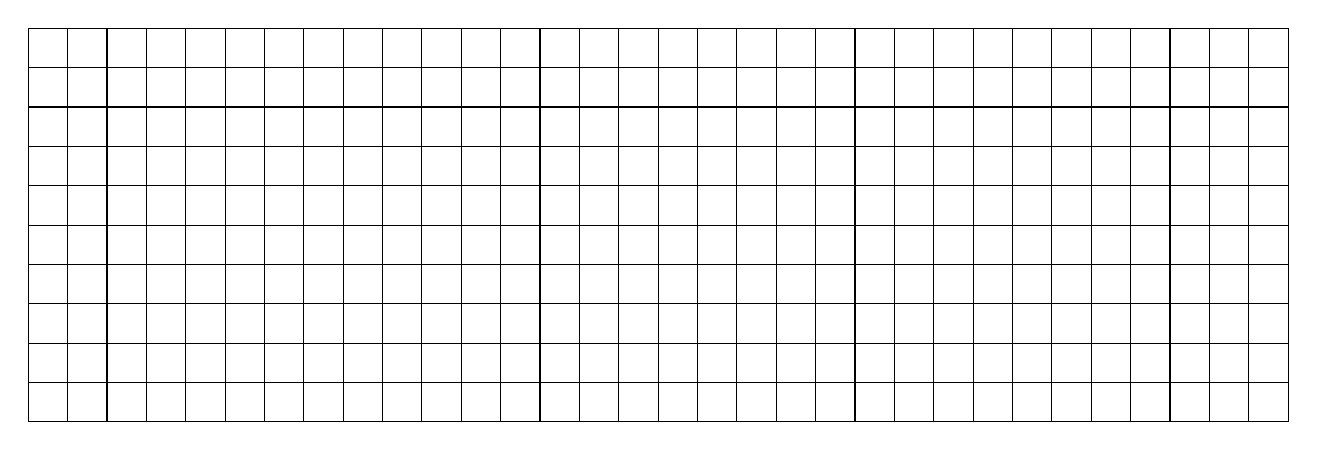
\begin{tikzpicture}
\draw[step=0.5,black,thin] (0,0) grid (16, 5);
\end{tikzpicture}
\end{center}

\textbf{(d)} Hence, or otherwise, Write an expression \emph{using indices} for the perimeter of stage $n$ as a multiple of the perimeter of stage 0 (so $4$ multiplied by something).

\vspace{0.1cm}
\begin{center}
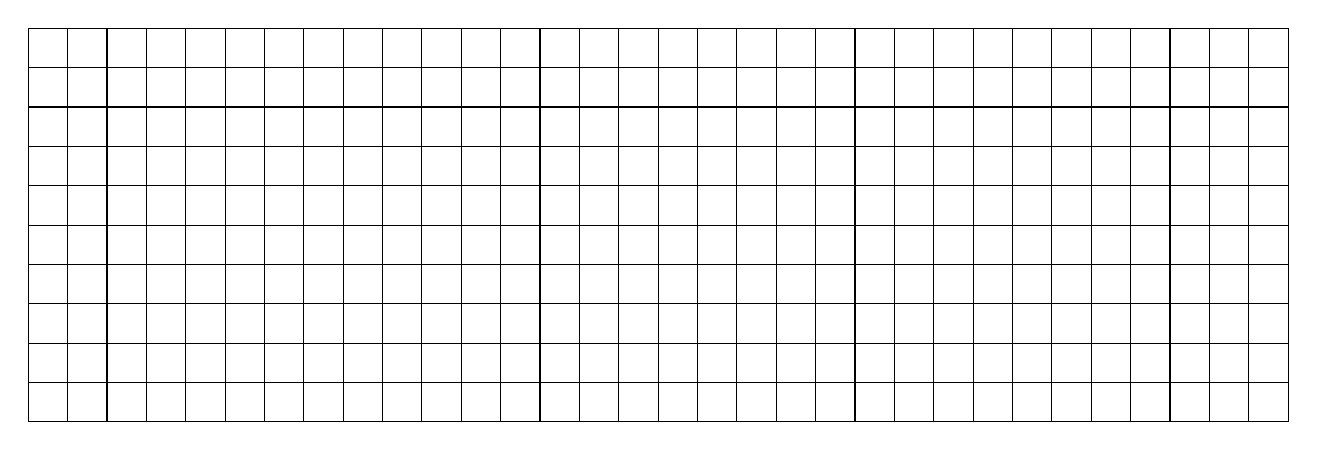
\begin{tikzpicture}
\draw[step=0.5,black,thin] (0,0) grid (16, 5);
\end{tikzpicture}
\end{center}

\textbf{(e)} Let $A_n$ represent the area (from part 1A (e)) and $P_n$ represent the perimeter (from part 1B (d)) of stage $n$. Find the perimeter-to-area ratio {\huge $\frac{P_n}{A_n}$}.

\vspace{0.1cm}
\begin{center}
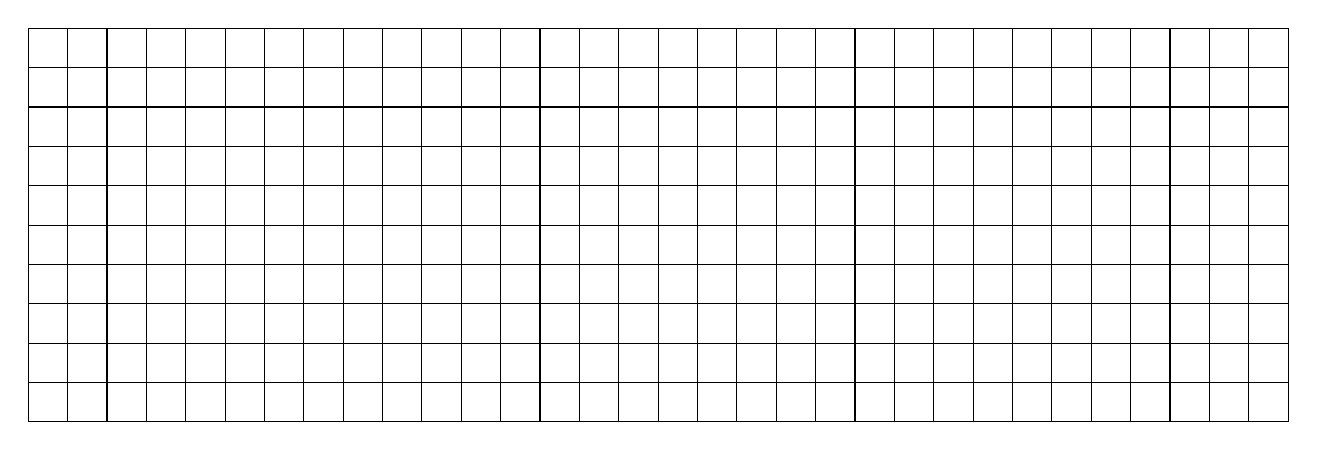
\begin{tikzpicture}
\draw[step=0.5,black,thin] (0,0) grid (16, 5);
\end{tikzpicture}
\end{center}





\pagebreak
{\Large \textbf{Part 2} \\[6pt]

In this part you will construct your own fractal. It can be based on a square (like this one), or a triangle, or another shape. \\[6pt]

\textbf{(a)} Draw the first 3 stages of your fractal.

\vspace{0.1cm}
\begin{center}
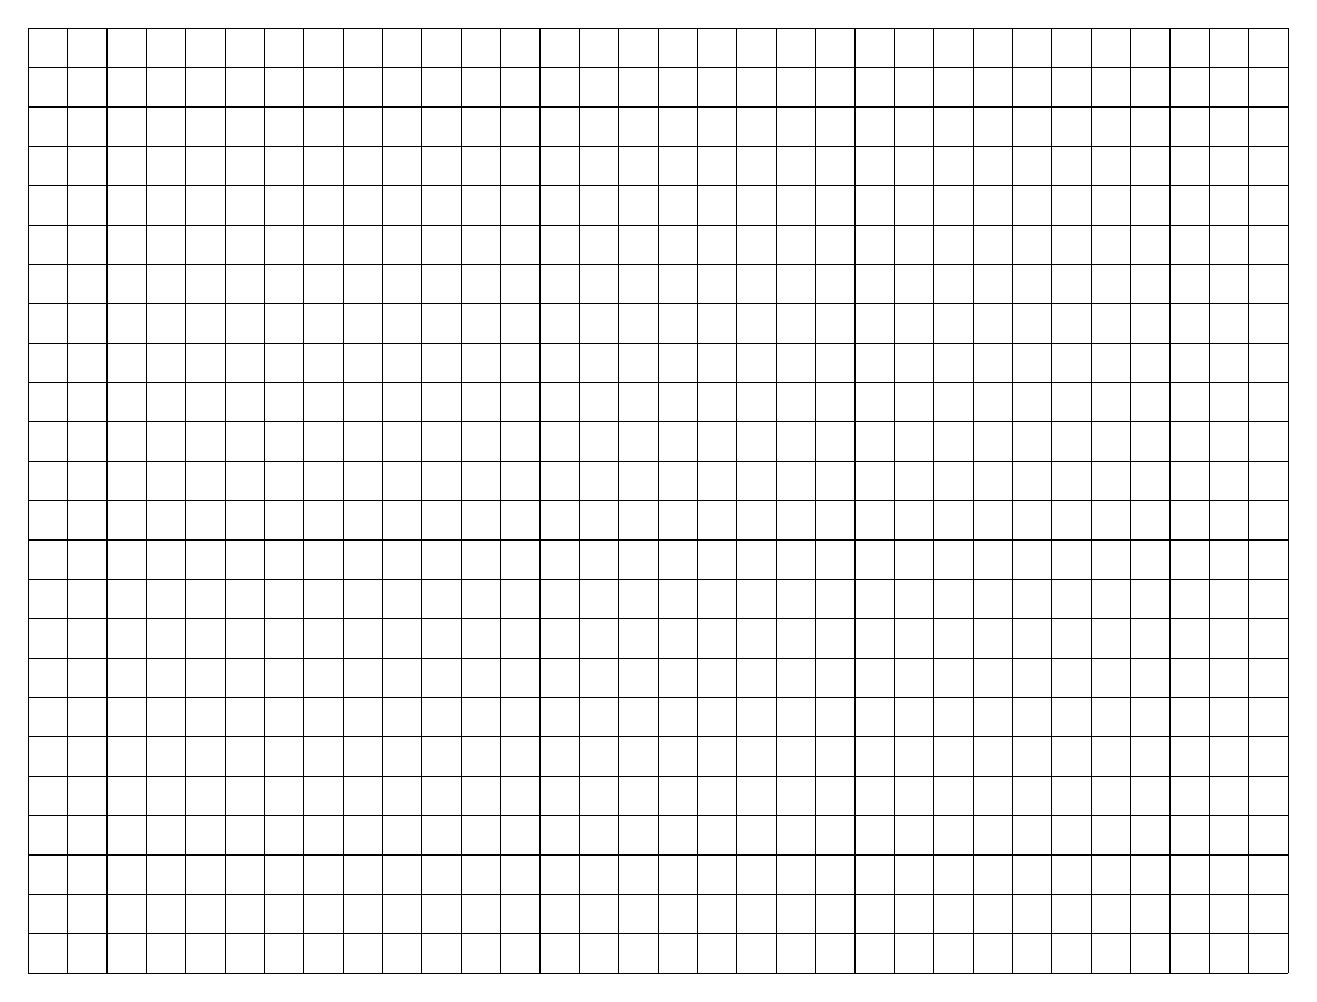
\begin{tikzpicture}
\draw[step=0.5,black,thin] (0,0) grid (16, 12);
\end{tikzpicture}
\end{center}

\textbf{(b)} Describe, in detail, how each stage of your fractal is constructed from the previous stage.

\vspace{0.4cm}
\begin{center}
\begin{tikzpicture}[scale=0.8]
\draw[black,thin] (0,0) -- (20, 0);
\draw[black,thin] (0,1) -- (20, 1);
\draw[black,thin] (0,2) -- (20, 2);
\draw[black,thin] (0,3) -- (20, 3);
\draw[black,thin] (0,4) -- (20, 4);
\draw[black,thin] (0,5) -- (20, 5);
\draw[black,thin] (0,6) -- (20, 6);
\end{tikzpicture}
\end{center}
\vspace{0.2cm}


\pagebreak
{\Large \textbf{Part 2 continued...} \\[6pt]

\textbf{(a)} Find an expression for the area of stage $n$ of your fractal.

\vspace{0.1cm}
\begin{center}
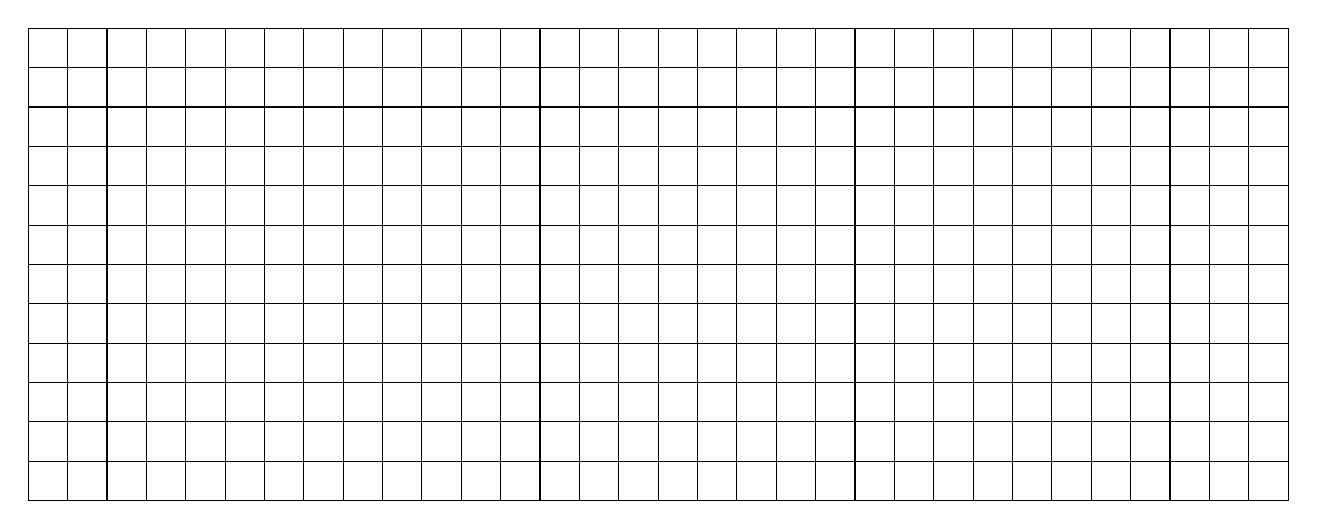
\begin{tikzpicture}
\draw[step=0.5,black,thin] (0,0) grid (16, 6);
\end{tikzpicture}
\end{center}

\textbf{(b)} Find an expression for the perimeter of stage $n$ of your fractal.

\vspace{0.1cm}
\begin{center}
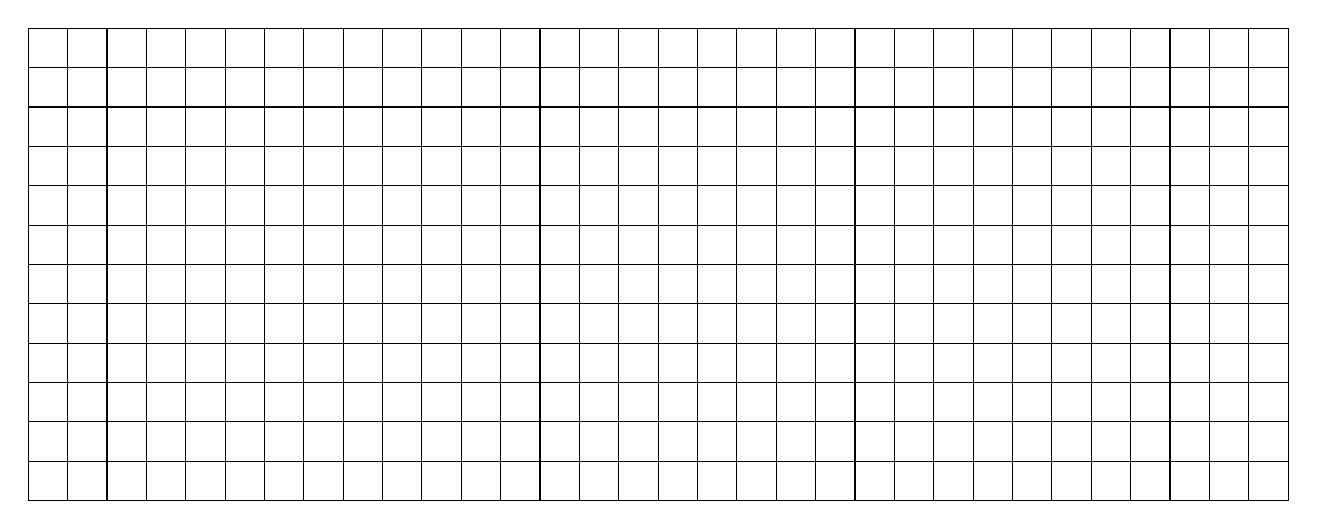
\begin{tikzpicture}
\draw[step=0.5,black,thin] (0,0) grid (16, 6);
\end{tikzpicture}
\end{center}

\textbf{(c)} Find an expression for the perimeter-to-area ratio of stage $n$ of your fractal.

\vspace{0.1cm}
\begin{center}
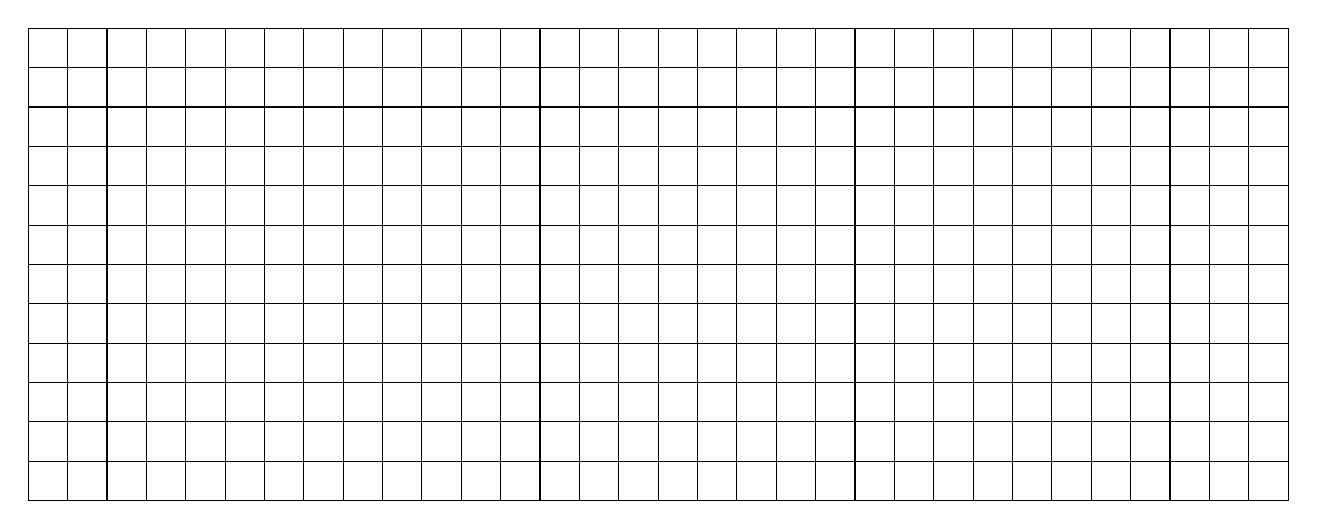
\begin{tikzpicture}
\draw[step=0.5,black,thin] (0,0) grid (16, 6);
\end{tikzpicture}
\end{center}



}


\end{document}
